\chapter{State of the Art}
\label{chapter:state_of_the_art}

Recently there have been an upsurge of interest in problems that require a combination of linguistic and visual information. Besides, the rise of social media in the web has made available a vast amount of multimodal information, like tagged photographs, illustrations in newspaper articles, videos with subtitles, and multimodal feeds on social media. To tackle combined language and vision tasks and to exploit the large amounts of multimodal information, the CV and NLP communities have been increasingly cooperating, for example by organizing combined workshops and conferences. One such area of research in the intersection of both worlds is automatic image description.

\textbf{Automatic image description} can be defined as the task of automatically generating a description of an image using natural language. It is a very challenging problem that combines two different problems into a single task: on the one hand, there is the problem of understanding an image, which belongs to the \textbf{Computer Vision (CV)} field, one the other hand, there is also the problem of generating a meaningful and grammatically-correct description of the image, which belongs to the \textbf{Natural-Language Processing (NLP)} field, and to be more precise, it belongs to the class of \textbf{Natural-Language Generation (NLG)} problems.

Both CV and NLP are challenging fields themselves. While both fields share common techniques rooted in artificial intelligence and machine learning, they have historically developed separately, with little interaction between their scientific communities.  Recent years have seen considerable advances in both fields, to a great extent thanks to the application of deep-learning techniques and the recent advances in this area. This chapter presents a brief survey of the recent literature on this topic, including some antecedents, but focusing primarily on the recent advances coming from the application of \textbf{Deep Learning} technology, since this is our main interest.

The chapter is organized in various sections. First section is devoted to further delimiting the task at hand as well as introducing classification system for the different approaches to the problem. Subsequent sections review relevant publications organized according to the provided classification scheme. Finally, there is a section describing the datasets used by the community to benchmark their models and a short discussion on the evaluation metrics for this kind of tasks.

\section{Task definition and overview}

We have already defined the task of automatic image description as the task of automatically generating a description of an image using natural language generation. However, this definition is too generic to precisely characterize the task we are interested in. For example, when presented with certain image, an algorithm may generate a list of labels describing different elements of the image, or it may describe technical features of the image, such as the dimensions, the predominant colors, brightness, etc. Therefore, we need a more concrete definition of the task.

When talking about \textbf{automatic image description}, we refer to descriptions that meet three properties:
\begin{itemize}
\item Descriptions that are relevant, that is, that talk about the elements of the image.
\item Descriptions that are expressed as natural language, using grammatically correct sentences
\item Descriptions that are comprehensive but concise at the same time, that is, the description should aim at summing up the important elements of the image, not just describing it.
\end{itemize}

From the CV point of view, this task requires \textbf{full image understanding}: the description should demonstrate or pretend a good understanding of the scene, far beyond simply recognizing the objects in the image. This means that the description is able to capture relations between the objects in the scene, and the actions happening there.

From the NLP point of view, this task requires \textbf{sophisticated natural language generation} (NLG), which involves: selecting which aspects to talk about (content selection), sorting and organizing the content to be verbalized (text planning), and finally generating a semantically and syntactically correct sentence (Surface realization).

Intuitively, descriptions should be easy to understand by a person, and that person should be able to grasp the essence of the image, to create a mental model of the image without actually seeing it. The description task can become even more challenging when we take into account user-specific tailored descriptions. For instance, when describing the paintings available in a museum, a tourist may require a different description than a librarian or an art critic.

Since 2011 there have been a considerable advance in challenging CV tasks, to a great extent fostered by the application of deep learning models and the availability of large corpus of data available to researchers. More recently, a similar process seems to be occurring in the NLP field. Not surprisingly, these advances in both CV and NLP have also propelled a new wave of interest in cross-disciplinary research problems involving both areas of research, and automatic image description is a very good example. As a consequence, the CV and NLP communities have increased cooperation, for example by organizing joint workshops over the past few years. These efforts have resulted in a surge of new models, datasets and evaluation measures, which is reflected in the increase of publications, specially from 2014. 

In order of ease of review, understanding and comparison of the growing amount of research on the topic, existing surveys have proposed various schemes to classify the models being used.
One the one hand, the survey by \citet{Bernardi2017} proposes a classification system based on two dimensions and only tree categories. On the other hand, \citet{Bai2018} organize the existing research according to the kind of architecture or framework used, resulting in a more fine grained classification with 8 categories. 

After comparing both both approaches to classify the existing research, we  prefer the approach adopted by \citet{Bai2018} as we consider it more precise and descriptive,  resulting in a finer granularity; while the classification by \cite{Bernardi2017} is more abstract, resulting in a coarser granularity. A more recent survey by \citet{Hossain2019} takes the same approach found in \citep{Bai2018} with a more focused review of deep-learning based models and references to the most recent work published so far.

Below we provide a short overview of the publications covered in this survey organized into categories and sorted by publication year:

\begin{table}[hpt]
    \caption{Summary of published research on the automatic image description problem}
    \label{tab:classification}
    \begin{tabular}{p{40mm}|p{120mm}}
        Approach & Representative research \\
        \hline
        Retrieval-based & \citet{Farhadi2010, Ordonez2011, Gupta2012, Kuznetsova2012, Hodosh2013a, Kuznetsova2014, Mason2015, Hodosh2013b}\\
        Template-based &  \citet{Yang2011, Kulkarni2011, Li2011, Mitchell2012, Ushiku2015}\\
        Earlier Deep Models &  \citet{Socher2014, Karpathy2014, Ma2016, Yan2015, Lebret2015a}\\
        Multimodal learning & \citet{Kiros2014a, Mao2015a, Karpathy2015, Chen2015}\\
        Compositional architectures & \citet{Fang2015, Tran2016, Ma2016, Oruganti2016, Wang2016, Fu2017},\\
        Attention-guided & \citet{Xu2015, You2016, Yang2016, Zhou2017, Cao2019, He2019}\\
        Describing novel objects & \citet{Mao2015b, Hendricks2016} 
    \end{tabular}
\end{table}

\section{Approaches without deep learning}

\subsection{Retrieval-based approaches}

Early work on the topic was often based in the use of retrieval-based approaches. These approaches usually follow a two steps process. During the first step, given a query image, a candidate set of similar images is retrieved using content-based image retrieval techniques, which are based on global image features extracted from the image. During the second step, a re-ranking of the retrieved images is computed using a variety of methods. Finally, the caption of the top image is returned, or a new caption is composed from the captions of the top-n ranked images.

\citet{Farhadi2010} use a meaning space consisting of \textit{<object, action, scene>} triplets to link images and sentences. Their model takes an input image, map it into the meaning space by solving a Markov Random Field, and use Lin's information-based similarity measure \citep{Lin1998} to determine the semantic distance between the query image and the pool of available captions. Finally, the semantically closest sentence is used as the image description.

The IM2TEXT model by \citet{Ordonez2011} uses the scene-centered descriptors of the GIST model \citep{Oliva2006, Torralba2008} to retrieve a set of similar images as a baseline, then these images are ranked using a classifier trained over a range of object detectors and scene classifiers specific to the entities mentioned in the candidate descriptions. Finally the caption of the top ranked image is returned. 

\citet{Kuznetsova2012} take on the work by \citet{Ordonez2011} with some notable twists: instead of retrieving a candidate set of images using content --visual-- features, their model start by running the detectors and scene classifiers used in the re-ranking step of the IM2TEXT model to extract and represent the semantic content of the query image. Then, instead of performing a single retrieval step to get neighbors of the query image, their model carries out a separate retrieval step for each visual entity detected in the query image. The result of this step is a collection of phrases of different type (noun and verb phrases and prepositional phrases). Finally, a new sentence is composed from a selected set of phrases using a constrain optimization approach. A refinement of the former approach is presented in \citet{Kuznetsova2014}, based on the use of tree structures to improve the sentence generation process.

\citet{Gupta2012} combine the image features of the GIST model with RGB and HSV color histograms, Gabor and Haar descriptors, and SIFT \citep{Lowe2004} descriptors for the retrieval step. Then, instead of using the visual features for the ranking step, their model relies on the textual descriptions of the retrieved images, which are segmented to obtain phrases of different type. This model takes the phrases associated to the retrieved images, rank them based on image similarity, and integrate them to get triples of the form \textit{( ((attribute1, object1), verb), (verb, prep, (attribute2, object2)), (object1, prep, object2) )}. Finally, the tree top-n triplets are used to generate an image description.

\citet{Hodosh2013b} employ a Kernel Canonical Correlation Analysis (KCCA) \citep{Bach2003} technique to project images and text items into a common space, where training images and their corresponding captions are maximally correlated. In the new common space, cosine similarities between images and sentences are calculated to rank the sentences, which are then used to select the top-n captions. This work is highly focused on the problems associated with existing benchmarks datasets and the evaluation metrics, and as a result the authors introduce a new dataset composed of 8000 images annotated with 5 captions per image, and propose a new metric based on binary judgments of image descriptions.

\citet{Mason2015} use visual similarity to retrieve a set of candidate captioned images. Second, a word probability density conditioned on the query image is computed from the retrieved captions. Finally, the candidate captions are scored using the word probability density and the one with the highest score is selected. 

An detailed analysis of the literature reviewed here reveals at least two dimensions that may further help in understanding and organizing the research: on the one hand, some approaches simply select one of the retrieved sentences as the image caption, while others compose a new caption by combining elements from several sentences; on the other hand, some approaches use visual detectors to find similar images (Content-Based Image Retrieval), while other approaches use conceptual information (Concept-Based Image Retrieval), or use a combination of visual and conceptual information for the retrieval step.

\begin{table}[hpt]
    \caption{Classification of retrieval-based automatic image captioning}
    \label{tab:retrieval-classification}
    \begin{tabular}{p{40mm}|p{60mm}|p{60mm}}
        Information modality & Select one caption & Compose caption \\
        \hline
        Visual & \citet{Farhadi2010, Mason2015} & \cite{Gupta2012} \\
        \hline
        Conceptual &  \cite{Ordonez2011} & \citet{Kuznetsova2012, Kuznetsova2014} \\
        \hline
        Hybrid &  \citet{Hodosh2013b}\\

    \end{tabular}
\end{table}

The main disadvantage of Retrieval-Based approaches comes from its reuse of existing images. The sentences used to describe images in the past may be completely inadequate for describing a new image. Although some of the proposed models are able to compose new sentences rather than just returning one of the stored sentences, these are still based on previously used sentences, so the result may still be unsuited for describing the query image. This limitation was specially evident with the use of small datasets, therefore, perhaps the problem would be alleviated with the use of very large datasets as the ones that have appeared recently \citet{Lin2014, Sharma2018}.

\section{Template-based approaches}

Another group of early attempts to solve the automatic image captioning problem take some kind of template-based approach. Unlike retrieval based approaches, template-based approaches analyze the query image to generate concepts, and then use some kind of constraining mechanism to compose a sentence. The constrains typically adopt the form of a template, but can also be specified as grammar rules.

For example, \citet{Yang2011} use a quadruplet consisting of \textit{<Noun-Verb-Scene-Preposition>} as template for generating image descriptions. The process starts with the execution of detection algorithms to estimate objects and scenes in the image, and then apply a language model trained over the Gigaword corpus\footnote{https://catalog.ldc.upenn.edu/LDC2003T05} to compute nouns, verbs, scenes and prepositions that might appear in the caption. Finally, they apply Hidden Markov Model Inference to compute probabilities for all the elements, and use the elements with the highest probabilities to fill the template and generate a new sentence.

\citet{Kulkarni2011} employ Conditional Random Field (CRF) to determine image contents, which results in a graph with nodes corresponding to objects in the image, object attributes, and spatial relationships between objects. Unary potential functions are computed for nodes in the graph, while pairwise potential functions are obtained on a collection of existing descriptions. Afterwards, CRF inference is used to determine the image contents to be described, and finally a sentence template is applied to generate sentence using the selected content.

\citet{Li2011} use visual models to detect objects, attributes and spatial relationships, and. Then, they resort to web-scale n-gram data to compute frequency counts of possible n-gram sequences to fill a triplet defined as \textit{<(adj1, obj1), prep, (adj2, obj2)>}. Finally, dynamic programming is applied to find an optimal set of phrases that constitute the description of the query image.

\citet{Mitchell2012} apply algorithms that are able to represent an image as an <objects, actions, spatial relationships> triplet. Syntactically informed word co-occurrence statistics are computed and used by a sentence generator to filter and constrain the output of the image processor using tree structures.

The aforementioned works in this section produce new sentences based on individual words (nouns, adjectives, verbs, prepositions, etc.) that generated in a piece-wise manner from the query image, and these words are later connected according to certain grammar model. To improve on this approach, some authors have proposed the use of phrases instead of individual words. In particular, \citet{Ushiku2015} present a method named Common Subspace for Model and Similarity (CoSMoS). CoSMoS obtains a subspace in which all feature vectors associated with the same phrase are mapped as mutually close, classifiers for each phrase are learned, and training samples are shared among co-occurring phrases. Phrases estimated from a query image are connected by using multi-stack beam search to generate a description.

Template-based approaches to automatic image captioning may improve the relevance of the resulting captions when compared with retrieval based approaches, template-based captions tend to be too rigid, thus resulting in a lack of naturality when compared to human-written sentences.

\section{Deep-learning approaches}

Convolutional Neural Networks (CNN) were first introduced by Yann LeCun in 1998 \citep{Lecun1998}, but it was not until more than a decade later than they started to shine. In 2012, a large, deep CNN \citep{Krizhevsky2012} was used to win, by a incredibly wide margin, the 2012 ImageNet Large-Scale Visual Recognition Challenge. From that turning point, the field has attracted attention of researchers from various fields and gained howling popularity. The success of CNN and other deep learning models was due to a great extent to its impressive results in many challenging problems, specially in the fields of Computer Vision and Natural Language Processing, where deep-learning models have became the state of the art. Not surprisingly, researchers have attempted to apply deep neural networks to solve problems in the interstice of both fields, CV and NLP, includes the problem of automatically generating image descriptions.

Recent advances in the field have been achieved with the introduction of new architectures and frameworks, accompanied by increasingly larger datasets to feed those deep neural networks. Therefore, there is a wide repertoire of methods for tackling the image captioning tasks. This section presents the contributions to the field organized according to the kind of architecture or framework utilized, with one subsection per category

\subsection{Earlier Deep Models}

Encourage by the success of CNNs to solve image classification tasks, researchers began incorporating deep models into their image captioning methods, yet still influenced by the retrieval-based and template-based methods. Image captioning was formulated as a multi-modality embedding \citet{Frome2013} and ranking problem.

\citet{Socher2014} use dependency-tree recursive neural networks (DT-RNN) to represent phrases and sentences as compositional vectors. Another deep neural network \citep{Le2011} is used to extract visual features from the images. Both types of  features are mapped into a common space by using a max-margin objective function. After training, sentence retrieval is performed based on similarities between representations of images and sentences in the common space.

\citet{Karpathy2014} introduce a twist in the previous model by working at a finer level, that is, instead of modelling full images, they work on a finer level by embedding fragments of images as well as fragments of sentences fragments into a common space.  An structured max-margin objective is used to explicitly associate these fragments across modalities. Image fragments are obtained by means of a Region CNN \citep{Girshick2014}. Sentence fragments are modelled as typed dependency tree relations \citep{DeMarneffe2006}. At last, a retrieval task is performed by computing image-sentence similarities that combine both a global term and a fragment-aligned term. Experimental evaluation showed that reasoning on both the global level of images and sentences and the finer level of their respective fragments improves performance on the image-sentence retrieval task.

\citet{Ma2015} take into consideration different levels of interaction between images and sentences in order to compute similarities. Their architecture combines two different deep neural networks to tackle the multimodal space: an image encoding CNN \citep{Simonyan2015} to encode visual data, and a matching CNN \citep{Hu2014} to learn the joint representation of images and sentences. The matching CNN composes words to different semantic fragments and learns the inter-modal relations between image and the composed fragments at different levels. The authors provide experimental results on benchmark databases for bidirectional image-sentence retrieval.

\subsection{Multimodal learning}

Retrieval-based and template-based methods to image captioning impose limitations on the capacity to describe images in the form of templates, structured prediction, and/or syntactic trees. Thanks to the advances in neural networks, new approaches emerged that were able to surpass those limitations. These methods can yield more expressive and flexible sentences with richer structures.  Multimodal neural language models constitute one way of approaching the problem from a learning perspective. In general, these models are bidirectional, that is, they are able to generate new captions for an image, but they can also be applied in retrieval tasks for both images and sentences.

\begin{figure}[hpt]
	\centering
	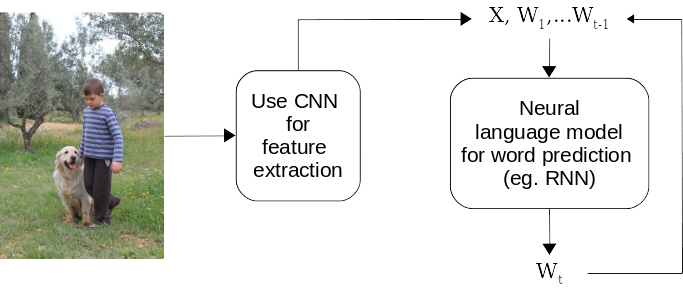
\includegraphics[scale=0.5]{ch2/multimodal.png}
	\caption{Structure of multimodal neural learning models for image captioning}
	\label{fig:multimodal}
\end{figure}

General structure of multimodal neural-based learning is shown in \ref{fig:multimodal}. First, image features are extracted using a feature extractor, typically a CNN. Then, the extracted features are forwarded to a neural-based model, which maps the image features into a common space with the word features. Finally, the model predicates new words based on the image feature and previously generated context words.

\citet{Kiros2014a} introduce two \textit{multimodal neural language models}: models of natural language that can be conditioned on other modalities. An image-text multimodal neural language model can be used to retrieve images given complex sentence queries, retrieve phrase descriptions given image queries, as well as generate text conditioned on images. The models used are adaptations of the log-bilinear language model proposed by \citep{Mnih2007}. In the case of image-text modelling it is possible to jointly learn word representations and image features by training the models together with a CNN. These models can be used for generating captions as well retrieval

\citet{Mao2014, Mao2015a} present a multimodal Recurrent Neural Network (m-RNN) model for generating novel image captions. It directly models the probability distribution of generating a word given previous words and an image, and uses this distribution to generate image captions. The model consists of two sub-networks: a deep RNN for sentences and a deep CNN for images. These two sub-networks interact with each other in a multimodal layer to form the whole m-RNN model. Besides generating captions, the m-RNN model can be applied for retrieving images or sentences. This model achieved state of art results across image captioning and image and caption retrieval tasks.

\citet{Karpathy2015} present a model that generates natural language descriptions of images and their regions by learning about the inter-modal correspondences between language and visual data. This model is based on a novel combination of CNN over image regions, bidirectional RNN over sentences, and a structured objective that aligns the two modalities through a multimodal embedding. The resulting Multimodal RNN architecture learns to generate novel descriptions of image regions. This model outperformed retrieval baselines on both full images and on a new dataset of region-level annotations derived from the MSCOCO dataset.
 
\citet{Chen2015} also explore the bi-directional mapping between images and their textual descriptions. This approach uses a RNN that attempts to dynamically build a visual representation of the scene as a caption is being generated or read. The representation automatically learns to remember long-term visual concepts. This model is capable of both generating novel captions given an image, and reconstructing visual features given an image description. The model was tested on several tasks, including sentence generation, sentence retrieval and image retrieval, and achieved state-of-the-art results for the task of generating novel image descriptions. The results for the image and sentence retrieval tasks were comparable to state-of-the-art methods using similar visual features.

\subsection{Encoder-Decoder framework}

Inspired by recent advances in neural machine translation, the encoder-decoder framework has also been applied with great success for generating image captions. General structure

\begin{figure}[hpt]
	\centering
	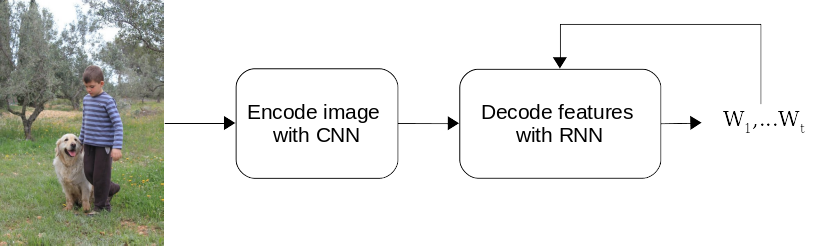
\includegraphics[scale=0.5]{ch2/encoder-decoder.png}
	\caption{Structure of image captioning methods based on the encoder-decoder framework}
	\label{fig:encoder-decoder}
\end{figure}

\subsection{Attention guided}

\begin{figure}[hpt]
	\centering
	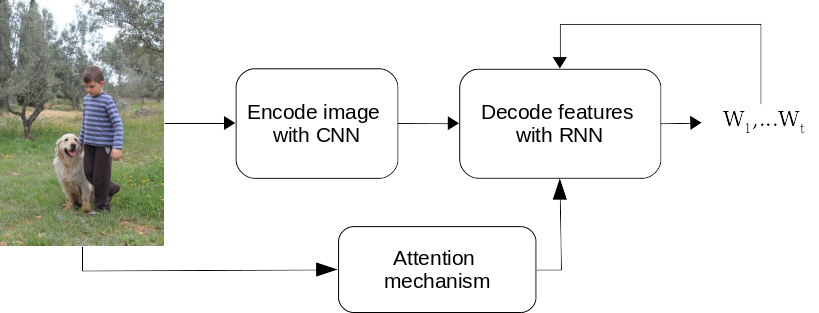
\includegraphics[scale=0.5]{ch2/attention-based.png}
	\caption{Structure of image captioning methods based on the encoder-decoder framework}
	\label{fig:attention-based}
\end{figure}

\subsection{Compositional architectures}

\begin{figure}[hpt]
	\centering
	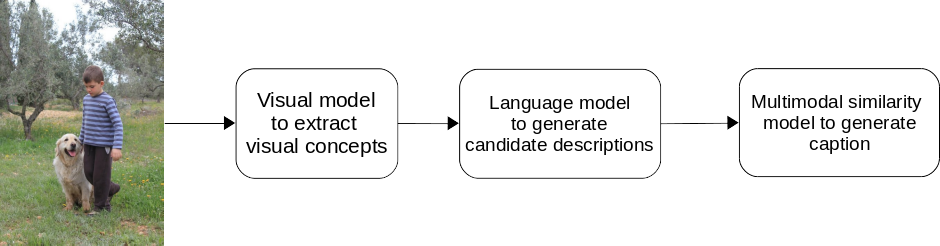
\includegraphics[scale=0.5]{ch2/compositional.png}
	\caption{Structure of image captioning methods based on the encoder-decoder framework}
	\label{fig:compositional}
\end{figure}

\subsection{Benchmark datasets and evaluation metrics}

\section{Datasets}

Pascal1K \citet{Rashtchian2010}

VLT2K \cite{Elliott2013}

Flickr8K \citet{Hodosh2015}

Flickr30K \cite{Young2014}

IAPTR-TC12 \cite{Grubinger2006}

MSCOCO \citet{Lin2014}

Conceptual Captions \cite{Sharma2018}

\section{Evaluation metrics}